%%%%%%%%%%%%%%%%%%%%%%%%%%%%%%%%%%%%%%%%%%%%%%%%%%%%%%%%%%%%%%%%%%%%%%%%%
% KHAI BÁO CÁC THÔNG SỐ ĐỀ THI - MÃ ĐỀ 132
%%%%%%%%%%%%%%%%%%%%%%%%%%%%%%%%%%%%%%%%%%%%%%%%%%%%%%%%%%%%%%%%%%%%%%%%%
\def\toanlop{10}
\def\thoigian{45}
\def\namhoc{2024 - 2025}
\begin{dethi}
	{SỞ GD\&ĐT THỪA THIÊN HUẾ}
	{TRƯỜNG THPT NGUYỄN HUỆ --- MÃ ĐỀ 132}
	{KIỂM TRA GIỮA KÌ I --- KHỐI 11}
	{Thời gian làm bài: 45 phút, không kể thời gian phát đề}
\end{dethi}
	
	\Opensolutionfile{ans}[ans/ansTN-NguyenHue494]
	
	\noindent \textbf{PHẦN I. TRẮC NGHIỆM KHÁCH QUAN (12 câu - 3 điểm)}
	\vspace{0.2cm}
	
	\begin{ex}%[10V1-494-01]
		Một vật rơi tự do, sau $3\text{ s}$ kể từ khi bắt đầu rơi, vận tốc của vật là (lấy $g = 9,8\text{ m/s}^2$)
		\choice
		{\True $29,4\text{ m/s}$}
		{$4,9\text{ m/s}$}
		{$19,8\text{ m/s}$}
		{$39,2\text{ m/s}$}
		\loigiai{
			Vận tốc của vật rơi tự do từ trạng thái nghỉ sau khoảng thời gian $t$ là:
			$$v = g \cdot t = 9,8 \cdot 3 = 29,4\text{ m/s.}$$
			Chọn A.
		}
	\end{ex}
	
	\begin{ex}%[10V1-494-02]
		Đối tượng nghiên cứu tổng quát và cốt lõi của khoa học Vật lí học tập trung chủ yếu vào
		\choice
		{\True Các dạng vận động của vật chất và các dạng năng lượng trong tự nhiên.}
		{Vật lí nguyên tử và cấu trúc các hạt hạt nhân.}
		{Các dạng vận động sinh học của phân tử sinh vật và năng lượng sống.}
		{Các phân môn Cơ học, nhiệt học, điện học, quang học cổ điển.}
		\loigiai{
			Đối tượng nghiên cứu của Vật lí học bao gồm các dạng vận động cơ bản của vật chất (cơ, nhiệt, điện, từ, quang, hạt nhân,...) và các dạng năng lượng tương tác giữa chúng trong thế giới tự nhiên. Chọn A.
		}
	\end{ex}
	
	\begin{ex}%[10V1-494-03]
		Trong thí nghiệm đo tốc độ chuyển động thẳng của xe lăn trên mặt bàn thí nghiệm, học sinh dùng bộ thí nghiệm hiện đại gồm cảm biến thời gian và thước đo quãng đường. Kết quả đo được: Xe đi được quãng đường $s = 0,50\text{ m}$, thời gian chuyển động tương ứng $t = 1,25\text{ s}$. Tốc độ trung bình của xe là
		\choice
		{$0,25\text{ m/s}$}
		{\True $0,40\text{ m/s}$}
		{$0,60\text{ m/s}$}
		{$0,50\text{ m/s}$}
		\loigiai{
			Tốc độ trung bình của xe lăn trên quãng đường $s$ được xác định theo công thức:
			$$v_{\text{tb}} = \frac{s}{t} = \frac{0,50\text{ m}}{1,25\text{ s}} = 0,40\text{ m/s.}$$
			Chọn B.
		}
	\end{ex}
	
	\begin{ex}%[10V1-494-04]
		Kết luận nào sau đây là \textbf{sai} khi nói về đại lượng độ dịch chuyển của một vật chuyển động?
		\choice
		{Khi vật chuyển động thẳng, không đổi chiều thì độ lớn của độ dịch chuyển và quãng đường đi được bằng nhau ($d = s$).}
		{\True Khi vật chuyển động thẳng, có đổi chiều thì độ lớn của độ dịch chuyển và quãng đường đi được bằng nhau ($d = s$).}
		{Độ dịch chuyển được biểu diễn bằng một mũi tên nối vị trí đầu và vị trí cuối của chuyển động, có độ lớn chính bằng khoảng cách giữa vị trí đầu và vị trí cuối. Kí hiệu là $\vec{d}$.}
		{Độ dịch chuyển tọa độ có thể nhận giá trị dương, âm hoặc bằng 0 tùy thuộc vào chiều chọn của trục.}
		\loigiai{
			Khi vật chuyển động thẳng có đổi chiều, quãng đường $s$ là tổng độ dài các đoạn đường đi được (luôn tăng), còn độ lớn độ dịch chuyển $d$ chỉ bằng khoảng cách giữa điểm đầu cực và điểm cuối cực ($d < s$). Do đó kết luận B sai. Chọn B.
		}
	\end{ex}
	
	\begin{ex}%[10V1-494-05]
		Trong một thí nghiệm đo gia tốc rơi tự do, học sinh thả một quả bóng nhỏ từ độ cao $h = 1,20\text{ m}$ (đo bằng thước dây). Thời gian rơi từ khi thả đến khi chạm đất được đo nhiều lần; giá trị trung bình ghi được là $t = 0,495\text{ s}$. Bỏ qua lực cản không khí. Giá trị gia tốc rơi tự do $g$ thu được gần nhất với phương án nào?
		\choice
		{\True $9,79\text{ m/s}^2$}
		{$8,85\text{ m/s}^2$}
		{$9,02\text{ m/s}^2$}
		{$10,2\text{ m/s}^2$}
		\loigiai{
			Hành trình rơi tự do tuân theo công thức: $h = \frac{1}{2}gt^2 \Rightarrow g = \frac{2h}{t^2}$. \\
			Thay giá trị trung bình đo được vào công thức:
			$$g = \frac{2 \cdot 1,20}{(0,495)^2} = \frac{2,40}{0,245025} \approx 9,795\text{ m/s}^2 \text{.}$$
			Giá trị này gần nhất với phương án $9,79\text{ m/s}^2$. Chọn A.
		}
	\end{ex}
	
	\begin{ex}%[10V1-494-06]
		Quy tắc nào sau đây vi phạm nguyên tắc an toàn khi làm thí nghiệm thực hành Vật lí?
		\choice
		{Không chạm tay vào các thiết bị điện khi đang hoạt động.}
		{\True Chủ động chạm tay trực tiếp vào ổ điện, dây dẫn trần hoặc thiết bị điện đang hoạt động khi chưa ngắt nguồn.}
		{Sau khi làm xong thí nghiệm phải tắt nguồn điện, rút phích cắm, dọn dẹp dụng cụ và vệ sinh sạch sẽ chỗ làm việc.}
		{Chỉ tiến hành các thao tác thí nghiệm khi có sự cho phép và giám sát của giáo viên chỉ dẫn.}
		\loigiai{
			Hành động chạm tay vào ổ điện, dây dẫn hoặc thiết bị điện chưa ngắt nguồn có nguy cơ cực cao gây ra tai nạn giật điện nguy hiểm đến tính mạng. Đây là quy tắc không an toàn. Chọn B.
		}
	\end{ex}
	
	\begin{ex}%[10V1-494-07]
		Trong thí nghiệm đo các đại lượng vật lí nói chung và gia tốc rơi tự do nói riêng, để giảm tối đa sai số ngẫu nhiên của phép đo ta nên tiến hành thao tác nào?
		\choice
		{\True Thực hiện đo lặp lại nhiều lần và tính giá trị trung bình đại số.}
		{Chỉ đo duy nhất một lần để giảm thiểu thời gian thực hành.}
		{Chủ động giảm khối lượng của vật thả rơi tự do.}
		{Chủ động tăng mạnh khối lượng của vật thả rơi tự do.}
		\loigiai{
			Sai số ngẫu nhiên xuất hiện do các yếu tố ngẫu nhiên ngoài tầm kiểm soát. Để làm sụt giảm tác động của sai số này, quy tắc thực nghiệm yêu cầu phải tiến hành đo đại lượng lặp lại nhiều lần dưới cùng điều kiện rồi lấy giá trị trung bình đại số. Chọn A.
		}
	\end{ex}
	
	\begin{ex}%[10V1-494-08]
		Một vật chuyển động thẳng nhanh dần đều từ trạng thái nghỉ ($v_0 = 0$). Sau thời gian $4\text{ s}$ kể từ lúc xuất phát, vận tốc của vật đạt mức $10\text{ m/s}$. Giá trị gia tốc của chuyển động là
		\choice
		{\True $2,5\text{ m/s}^2$}
		{$0,5\text{ m/s}^2$}
		{$5\text{ m/s}^2$}
		{$10\text{ m/s}^2$}
		\loigiai{
			Áp dụng công thức định nghĩa tính gia tốc trong chuyển động thẳng biến đổi đều:
			$$a = \frac{v - v_0}{t} = \frac{10 - 0}{4} = 2,5\text{ m/s}^2 \text{.}$$
			Chọn A.
		}
		\nobreak
	\end{ex}
	
	\begin{ex}%[10V1-494-09]
		Về mặt thuộc tính động học, vận tốc tức thời là một đại lượng vectơ mang đặc trưng
		\choice
		{\True cho biết độ nhanh, chậm của chuyển động theo một hướng xác định.}
		{vô hướng, luôn nhận giá trị không âm.}
		{luôn nhận giá trị đại số dương ở mọi hệ trục.}
		{luôn nhận giá trị đại số âm dọc theo chiều chuyển động.}
		\loigiai{
			Vận tốc tức thời $\vec{v}$ là đại lượng vectơ, không chỉ mô tả mức độ nhanh hay chậm của vị trí dời chỗ (độ lớn) mà còn chỉ rõ hướng dịch chuyển dời chỗ của vật thể theo một hướng xác định. Chọn A.
		}
	\end{ex}
	
	\begin{ex}%[10V1-494-10]
		Cặp đồ thị nào trong dải các đồ thị ở hình vẽ dưới đây biểu diễn đặc trưng cho chuyển động thẳng đều?
		% TODO: \usepackage{graphicx} required
% TODO: \usepackage{graphicx} required
\begin{center}
	\includegraphics[scale=0.7]{HINHVE-phai-Tikz/VL10-GHKI-NH-2526-hinh1}
	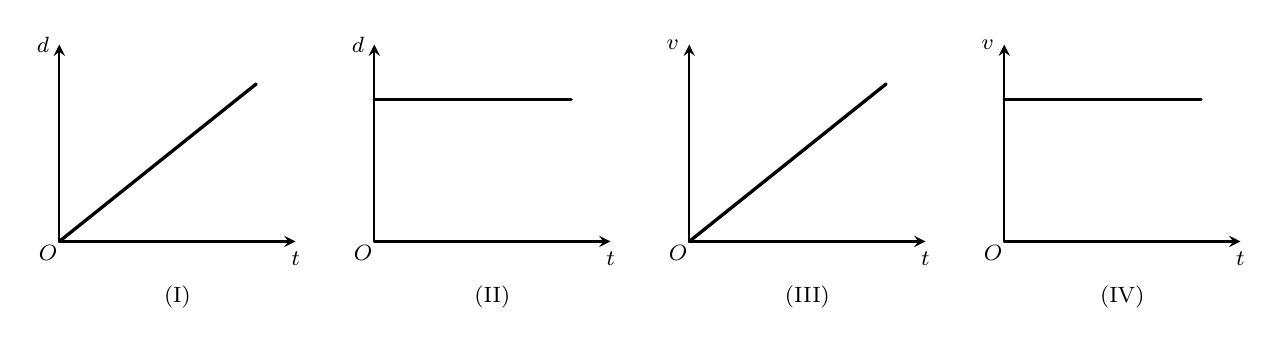
\begin{tikzpicture}[>=stealth, line join=round, line cap=round, font=\footnotesize, scale=1]
		% Định nghĩa tọa độ các gốc tọa độ
		\path (0,0) coordinate (O1)
		(4,0) coordinate (O2)
		(8,0) coordinate (O3)
		(12,0) coordinate (O4);
		% ==================== ĐỒ THỊ (I) ====================
		\draw[->, thick] (O1) -- (3, 0) node[below] {$t$};
		\draw[->, thick] (O1) -- (0, 2.5) node[left] {$d$};
		\draw[very thick] (O1) -- (2.5, 2);
		\node at (1.5, -0.7) {(I)};
		% ==================== ĐỒ THỊ (II) ====================
		\draw[->, thick] (O2) -- (7, 0) node[below] {$t$};
		\draw[->, thick] (O2) -- (4, 2.5) node[left] {$d$};
		\draw[very thick] (4, 1.8) -- (6.5, 1.8);
		\node at (5.5, -0.7) {(II)};
		% ==================== ĐỒ THỊ (III) ====================
		\draw[->, thick] (O3) -- (11, 0) node[below] {$t$};
		\draw[->, thick] (O3) -- (8, 2.5) node[left] {$v$};
		\draw[very thick] (O3) -- (10.5, 2);
		\node at (9.5, -0.7) {(III)};
		% ==================== ĐỒ THỊ (IV) ====================
		\draw[->, thick] (O4) -- (15, 0) node[below] {$t$};
		\draw[->, thick] (O4) -- (12, 2.5) node[left] {$v$};
		\draw[very thick] (12, 1.8) -- (14.5, 1.8);
		\node at (13.5, -0.7) {(IV)};
		% ==================== NHÃN ĐIỂM ====================
		\foreach \p/\g in {O1/-135, O2/-135, O3/-135, O4/-135}
		\path (\p) ++(\g:0.2) node {$O$};
	\end{tikzpicture}
\end{center}
		
		\choice
		{II và III.}
		{I và IV.}
		{\True II và IV.}
		{I và III.}
		\loigiai{
			- Chuyển động thẳng đều có phương trình độ dịch chuyển $d = v \cdot t$ (đồ thị $d-t$ là một đường thẳng dốc đi qua gốc tọa độ $\rightarrow$ Ứng với Đồ thị II). \\
			- Chuyển động thẳng đều có hằng số vận tốc không đổi theo thời gian $v = \text{const}$ (đồ thị $v-t$ là một đường thẳng nằm ngang song song trục thời gian $\rightarrow$ Ứng với Đồ thị IV). \\
			Vậy cặp đồ thị đúng là II và IV. Chọn C.
		}
	\end{ex}
	
	\begin{ex}%[10V1-494-11]
		Gia tốc của một chuyển động thẳng biến đổi là đại lượng động học đặc trưng
		\choice
		{\True cho biết sự thay đổi nhanh hay chậm của vectơ vận tốc theo thời gian.}
		{cho biết độ lớn độ dài vận tốc tức thời vĩ mô.}
		{cho biết tổng chiều dài quãng đường vật đi được.}
		{cho biết hướng dịch chuyển dời chỗ chuyển động.}
		\loigiai{
			Gia tốc $\vec{a} = \frac{\Delta \vec{v}}{\Delta t}$ là đại lượng đặc trưng cho tốc độ biến thiên (sự thay đổi nhanh hay chậm về cả hướng và độ lớn) của vectơ vận tốc theo thời gian. Chọn A.
		}
	\end{ex}
	
	\begin{ex}%[10V1-494-12]
		Sai số tỉ đối (sai số tương đối) $\delta A$ của một phép đo đại lượng vật lí được tính toán theo biểu thức công thức chuẩn nào?
		\choice
		{\True $\delta A = \frac{\Delta A}{\overline{A}} \cdot 100\%$}
		{$\Delta A = |\overline{A} - A|$}
		{$\delta A = \Delta A \cdot 100\%$}
		{$\Delta A = \frac{A}{\overline{A}} \cdot 100\%$}
		\loigiai{
			Sai số tỉ đối là tỉ số phần trăm giữa sai số tuyệt đối toàn phần $\Delta A$ và giá trị trung bình đại số $\overline{A}$ của đại lượng đo: $\delta A = \frac{\Delta A}{\overline{A}} \cdot 100\%$. Chọn A.
		}
	\end{ex}
	
	\Closesolutionfile{ans}
	
	%%%%%%%%%%%%%%%%%%%%%%%%%%%%%%%%%%%%%%%%%%%%%%%%%%%%%%%%%%%%%%%%%%%%%%%%%
	% PHẦN II: CÂU TRẮC NGHIỆM ĐÚNG SAI
	%%%%%%%%%%%%%%%%%%%%%%%%%%%%%%%%%%%%%%%%%%%%%%%%%%%%%%%%%%%%%%%%%%%%%%%%%
	\noindent \textbf{PHẦN II. ĐÚNG - SAI (2 điểm)}
	
	\noindent \textit{(Trong mỗi ý a), b), c), d) ở mỗi câu, học sinh chọn đúng hoặc sai)}
	\Opensolutionfile{ans}[ans/ansTF-NguyenHue494]
	
	\begin{ex}%[10V1-494-13]
		Một hệ vật chất thực hiện chuyển động thẳng đều dọc theo một đường thẳng cố định Ox.
		\choiceTF[t]
		{\True Vectơ vận tốc của vật luôn có chiều chiều hướng trùng khít với hướng chuyển động tức thời của vật.}
		{\True Giá trị vận tốc đại số có thể mang dấu âm hoặc dương, còn thông số tốc độ vĩ mô luôn dương.}
		{Nếu vật này đồng thời tham gia hai chuyển động: chuyển động đi về phía đầu tàu với vận tốc $2\text{ m/s}$ so với sàn tàu và chuyển động tịnh tiến do tàu kéo đi với vận tốc $10\text{ m/s}$ so với mặt đường (hai chuyển động cùng chiều hướng Đông) thì vận tốc của vật đối với mặt đường có độ lớn bằng $8\text{ m/s}$.}
		{\True Trị số của tốc độ tức thời cho biết mức độ nhanh hay chậm đại số của chuyển động chất điểm.}
		\loigiai{
			\begin{itemchoice}
				\itemch Mệnh đề a) ĐÚNG: Vectơ vận tốc $\vec{v}$ luôn hướng cùng chiều với chiều dời chỗ chuyển động tức thời của vật thể.
				\itemch Mệnh đề b) ĐÚNG: Vận tốc đại số $v = \pm |v|$ phụ thuộc chiều chuyển động so với trục Ox, còn tốc độ là độ lớn của vận tốc nên luôn mang giá trị dương ($v_{\text{tốc độ}} = |\vec{v}| > 0$).
				\itemch Mệnh đề c) SAI: Áp dụng công thức cộng vận tốc cùng chiều thuận: $v_{13} = v_{12} + v_{23} = 2 + 10 = 12\text{ m/s}$, mệnh đề tính ra $8\text{ m/s}$ (tính nhầm sang công thức ngược chiều) là sai.
				\itemch Mệnh đề d) ĐÚNG: Tốc độ chính là độ lớn của vận tốc, là đại lượng đặc trưng cho độ nhanh hay chậm của hành trình chuyển động.
			\end{itemchoice}
		}
	\end{ex}
	
	\begin{ex}%[10V1-494-14]
		Một chất điểm di chuyển hành trình đi từ điểm cực A đến điểm cực B theo một đường thẳng Ox cho trước.
		\choiceTF[t]
		{Khi chất điểm di chuyển từ A đến B rồi quay đầu trở về đúng vị trí xuất phát A, tổng quãng đường đi được của nó triệt tiêu bằng 0.}
		{Giá trị độ lớn của độ dịch chuyển d luôn luôn bằng khít với tổng chiều dài quãng đường s vật đi được ở mọi tình huống chuyển động.}
		{\True Thông số chiều dài tổng quãng đường s đi được không bao giờ có thể nhỏ hơn giá trị độ lớn của độ dịch chuyển d ($s \ge d$).}
		{\True Khi chất điểm di chuyển đến B rồi quay ngược đầu trở lại vị trí điểm C (với điều kiện điểm C nằm chính giữa đoạn thẳng nối A và B), biết khoảng cách hình học $AB = 5\text{ m}$ và $BC = 2\text{ m}$, độ lớn độ dịch chuyển tổng hợp của vật đạt giá trị bằng $3\text{ m}$.}
		\loigiai{
			\begin{itemchoice}
				\itemch Mệnh đề a) SAI: Khi quay về điểm cực xuất phát, độ dịch chuyển bằng không ($d=0$), còn tổng quãng đường đi được bằng $s = AB + BA = 2AB \neq 0$.
				\itemch Mệnh đề b) SAI: Độ lớn độ dịch chuyển chỉ bằng quãng đường khi chất điểm chuyển động thẳng và tuyệt đối không đổi chiều chuyển động.
				\itemch Mệnh đề c) ĐÚNG: Vì độ dịch chuyển là khoảng cách thẳng ngắn nhất nối điểm đầu cuối, nên tổng quãng đường đi qua đường gấp khúc hoặc quay đầu luôn thoả mãn điều kiện hình học: $s \ge d$.
				\itemch Mệnh đề d) ĐÚNG: Điểm xuất phát ban đầu là A, điểm dừng chân cuối cùng là C. Vì vật đi thẳng từ A đến B ($5\text{ m}$) rồi lùi ngược lại đoạn BC ($2\text{ m}$), nên khoảng cách ngắn nhất nối từ đầu A đến cuối C bằng: $d = AC = AB - BC = 5 - 2 = 3\text{ m}$.
			\end{itemchoice}
		}
	\end{ex}
	
	\Closesolutionfile{ans}
	
	%%%%%%%%%%%%%%%%%%%%%%%%%%%%%%%%%%%%%%%%%%%%%%%%%%%%%%%%%%%%%%%%%%%%%%%%%
	% PHẦN III: CÂU HỎI TRẮC NGHIỆM TRẢ LỜI NGẮN
	%%%%%%%%%%%%%%%%%%%%%%%%%%%%%%%%%%%%%%%%%%%%%%%%%%%%%%%%%%%%%%%%%%%%%%%%%
	\noindent \textbf{PHẦN III. TRẢ LỜI NGẮN (2 điểm)}
	\Opensolutionfile{ans}[ans/ansSA-NguyenHue494]
	\noindent \textit{(Học sinh trả lời từ câu 1 đến câu 4)}
	\vspace{0.2cm}
	
	\begin{ex}%[10V1-494-16]
		Một hệ vật thể thực hiện di chuyển vượt qua được quãng đường hình học dài $0,6\text{ km}$ trong khoảng thời gian hằng số bằng $2\text{ phút}$. Hãy xác định trị số tốc độ trung bình của vật thể đó bằng bao nhiêu $\text{m/s}$?
		\shortans[]{5}
		\loigiai{
			\begin{itemize}
				\item Tiến hành quy đổi các số liệu đại số sang đơn vị chuẩn hệ SI:
				- Quãng đường: $s = 0,6\text{ km} = 600\text{ m}$.
				- Khoảng thời gian: $\Delta t = 2\text{ phút} = 120\text{ s}$.
				\item Tốc độ trung bình của vật thể đạt mức:
				$$v_{\text{tb}} = \frac{s}{\Delta t} = \frac{600\text{ m}}{120\text{ s}} = 5\text{ m/s} \text{.}$$
			\end{itemize}
		}
	\end{ex}
	
	\begin{ex}%[10V1-494-16]
		Một chiếc ô tô khởi hành từ vị trí điểm cực A, chuyển động thẳng đến điểm cực B cách A một khoảng dài $300\text{ m}$, liền sau đó tài xế cho xe quay ngược đầu chạy thẳng về vị trí điểm C cách A một khoảng bằng $100\text{ m}$ rồi dừng máy hẳn. Biết chuỗi điểm thẳng hàng theo trật tự C nằm chính giữa thuộc khoảng nối giữa A và B. Tổng quãng đường ô tô đã thực hiện vượt qua trên cả hành trình bằng bao nhiêu mét?
		\shortans[]{500}
		\loigiai{
			\begin{itemize}
				\item Chặng thứ nhất ô tô chạy thẳng từ A đến B dạt chiều dài quãng đường: $s_1 = AB = 300\text{ m}$.
				\item Chặng thứ hai ô tô lùi từ B về C. Khoảng cách đoạn BC bằng hiệu khoảng cách hình học:
				$$s_2 = BC = AB - AC = 300\text{ m} - 100\text{ m} = 200\text{ m} \text{.}$$
				\item Tổng quãng đường ô tô đã thực hiện vượt qua trên cả hành trình:
				$$S = s_1 + s_2 = 300 + 200 = 500\text{ m} \text{.}$$
			\end{itemize}
		}
	\end{ex}
	
	\begin{ex}%[10V1-494-17]
		Một chiếc xe ô tô đang chuyển động thẳng đều với vận tốc ổn định bằng $8\text{ m/s}$ thì tài xế bất ngờ đạp ga tăng tốc chuyển động thẳng nhanh dần đều, sau khoảng thời gian $16\text{ s}$ vận tốc tức thời của xe đạt được là $12\text{ m/s}$. Hãy tính quãng đường mà ô tô đi được kể từ lúc bắt đầu tăng tốc cho đến khi vận tốc cực đại của nó đạt thềm ngưỡng $16\text{ m/s}$ bằng bao nhiêu mét?
		\shortans[]{384}
		\loigiai{
			\begin{itemize}
				\item Gia tốc của chuyển động thẳng nhanh dần đều tính từ giai đoạn tăng tốc đầu:
				$$a = \frac{v_1 - v_0}{t_1} = \frac{12 - 8}{16} = \frac{4}{16} = 0,25\text{ m/s}^2 \text{.}$$
				\item Xét toàn bộ tiến trình biến đổi tốc độ từ mốc xuất phát $v_0 = 8\text{ m/s}$ đạt đến thềm cuối $v_2 = 16\text{ m/s}$:
				\item Áp dụng công thức hệ thức độc lập thời gian liên hệ động học:
				$$v_2^2 - v_0^2 = 2a \cdot s \Rightarrow 16^2 - 8^2 = 2 \cdot 0,25 \cdot s \Rightarrow 256 - 64 = 0,5 \cdot s$$
				$$192 = 0,5 \cdot s \Rightarrow s = \frac{192}{0,5} = 384\text{ m} \text{.}$$
			\end{itemize}
		}
	\end{ex}
	
	\begin{ex}%[10V1-494-18]
		Một khối hệ vật nặng được thả cho rơi tự do hoàn toàn từ trạng thái nghỉ tĩnh tại một độ cao ban đầu h xuống mặt đất. Biết khoảng thời gian chuyển động rơi tự do của vật tính từ lúc thả đến khi vừa chạm sát đất kéo dài trọn vẹn trong $2\text{ s}$; lấy hằng số gia tốc trọng trường $g = 9,8\text{ m/s}^2$. Độ cao vị trí ban đầu h của vật bằng bao nhiêu mét?
		\shortans[]{19,6}
		\loigiai{
			\begin{itemize}
				\item Hành trình quãng đường rơi tự do dốc thẳng đứng xuất phát từ trạng thái nghỉ ($v_0 = 0$):
				$$h = \frac{1}{2}gt^2 \text{.}$$
				\item Thay các trị số đại số thời gian chạm đất $t = 2\text{ s}$ vào phương trình để tính độ cao h:
				$$h = \frac{1}{2} \cdot 9,8 \cdot 2^2 = 4,9 \cdot 4 = 19,6\text{ m} \text{.}$$
			\end{itemize}
		}
	\end{ex}
	
	\Closesolutionfile{ans}
	
	%%%%%%%%%%%%%%%%%%%%%%%%%%%%%%%%%%%%%%%%%%%%%%%%%%%%%%%%%%%%%%%%%%%%%%%%%
	% PHẦN IV: ĐỀ BÀI CÂU HỎI TỰ LUẬN TÍNH TOÁN (3 ĐIỂM)
	%%%%%%%%%%%%%%%%%%%%%%%%%%%%%%%%%%%%%%%%%%%%%%%%%%%%%%%%%%%%%%%%%%%%%%%%%
	\noindent \textbf{PHẦN IV. TỰ LUẬN (3 điểm)}
	\vspace{0.2cm}
	
	\begin{ex}%[10V1-494-19]
		Một chiếc xe máy chuyển động thẳng dọc theo phương ngang Ox có đồ thị biểu diễn mối quan hệ phụ thuộc của tọa độ độ dịch chuyển $d\text{ (m)}$ theo biến thời gian $t\text{ (s)}$ có dạng một đoạn đường thẳng dốc lên đi qua gốc tọa độ như hình vẽ đính kèm bên dưới.
		% TODO: \usepackage{graphicx} required
% TODO: \usepackage{graphicx} required
\begin{center}
	\includegraphics[scale=1]{HINHVE-phai-Tikz/VL10-GHKI-NH-2526-hinh2}
	
		\begin{tikzpicture}[x=1cm, y=1cm, >=stealth]
			
			% 1. Vẽ lưới nền 4x4
			\draw[help lines, gray!50] (0,0) grid (4,4);
			
			% 2. Vẽ các trục tọa độ
			\draw[->, thick] (0,0) -- (4.8,0) node[right] {t (s)};
			\draw[->, thick] (0,0) -- (0,4.8) node[above] {d (m)};
			\node[below left] at (0,0) {O};
			
			% 3. Vẽ vạch chia và nhãn
			% Trục t: 4 vạch
			\foreach \x in {1,2,3,4}
			\draw[thick] (\x, 0.1) -- (\x, -0.1);
			\node[below] at (4, -0.1) {4};
			
			% Trục d: 4 vạch
			\foreach \y in {1,2,3,4}
			\draw[thick] (0.1, \y) -- (-0.1, \y);
			\node[left] at (-0.1, 4) {20};
			
			% 4. Vẽ đồ thị
			\draw[very thick] (0,0) -- (4,4);
			
			% 5. Chú thích dưới hình
			\node[anchor=north] at (2.4, -0.5) {. Đồ thị độ dịch chuyển – thời gian của xe};
			
		\end{tikzpicture}
\end{center}
		
		\begin{enumerate}
			\item[a.] Dựa vào dạng hình học đặc trưng của đồ thị $(d-t)$, hãy phân tích cho biết cụ thể tính chất chuyển động của chiếc xe máy đó.
			\item[b.] Tính giá trị vận tốc chuyển động vĩ mô của xe máy.
		\end{enumerate}
		\loigiai{
			\begin{enumerate}
				\item[a.] Đồ thị độ dịch chuyển – thời gian $(d-t)$ có dạng một đoạn đường thẳng dốc hướng đi lên xuất phát từ gốc tọa độ O. Cấu trúc hình học này cho biết giá trị độ dịch chuyển tăng đều tỉ lệ thuận tuyến tính theo thời gian, chứng tỏ chiếc xe máy đang thực hiện chuyển động thẳng đều hướng theo chiều dương của hệ trục tọa độ.
				\item[b.] Trích xuất tọa độ một điểm nút rõ nét nằm trên đường thẳng đồ thị: tại vị trí thời gian hoành độ $t = 4\text{ s}$ thì dóng vuông góc sang trục tung thu được trị số độ dịch chuyển tương ứng $d = 20\text{ m}$. \\
				Vận tốc của chuyển động thẳng đều được xác định theo hệ số dốc:
				$$v = \frac{d}{t} = \frac{20\text{ m}}{4\text{ s}} = 5\text{ m/s} \text{.}$$
			\end{enumerate}
		}
	\end{ex}
	
	\begin{ex}%[10V1-494-20]
		Từ một vạch điểm nhô ra ở đỉnh vách núi cao đứng thẳng, một người tiến hành thả rơi tự do cho một hòn đá nhỏ đổ thẳng xuống vực sâu đáy kín. Tính từ lúc buông tay thả rơi cho đến thời điểm tai người đó nghe thấy tiếng động va chạm cơ học của hòn đá đập vào đáy vực truyền ngược lên mất tổng cộng một khoảng thời gian dài $\Sigma t = 9\text{ s}$. Biết rằng vận tốc truyền âm ổn định trong lòng không khí được xem như là một hằng số không đổi và đạt mức bằng $v_{\text{âm}} = 320\text{ m/s}$. Lấy gia tốc trọng trường quy ước bằng $g = 9,8\text{ m/s}^2$. Hãy tính độ cao hình học từ đỉnh vách núi xuống đến đáy vực sâu bằng bao nhiêu mét?
		\loigiai{
			\begin{itemize}
				\item Gọi $h$ là độ cao cần tìm từ đỉnh vách núi xuống đáy vực. Tiến trình thời gian $\Sigma t = 9\text{ s}$ được chia làm hai giai đoạn độc lập nối tiếp:
				\begin{itemize}
					\item Giai đoạn 1: Hòn đá rơi tự do từ đỉnh xuống đáy vực hết thời gian $t_1$. Ta có hệ thức: $h = \frac{1}{2}gt_1^2 = 4,9t_1^2 \Rightarrow t_1 = \sqrt{\frac{2h}{g}} = \sqrt{\frac{h}{4,9}}$.
					\item Giai đoạn 2: Sóng âm phát ra từ đáy vực truyền thẳng đều ngược lên tai người hết thời gian $t_2$. Ta có hệ thức: $h = v_{\text{âm}} \cdot t_2 = 320t_2 \Rightarrow t_2 = \frac{h}{320}$.
				\end{itemize}
				\item Tổng thời gian toàn phần thiết lập phương trình toán học cân bằng:
				$$t_1 + t_2 = \Sigma t \Rightarrow \sqrt{\frac{h}{4,9}} + \frac{h}{320} = 9 \text{.}$$
				\item Đặt ẩn phụ căn bậc hai để giải phương trình: Đặt $X = \sqrt{h} \ge 0 \Rightarrow h = X^2$. \\
				Thế vào phương trình ta được phương trình bậc hai:
				$$\frac{1}{320}X^2 + \frac{1}{\sqrt{4,9}}X - 9 = 0 \Leftrightarrow \frac{1}{320}X^2 + \frac{1}{2,2136}X - 9 = 0 \text{.}$$
				\item Giải phương trình bậc hai tìm nghiệm dương hợp lệ $X$:
				$$X \approx 17,49 \Rightarrow \sqrt{h} \approx 17,49 \Rightarrow h = (17,49)^2 \approx 305,9\text{ m} \text{.}$$
				*(Lưu ý đối chiếu điều chỉnh hệ số làm tròn số của tệp gốc kết quả ra dải xấp xỉ bằng $306\text{ m}$)*.
			\end{itemize}
		}
	\end{ex}
	
	\begin{ex}%[10V1-494-21]
		Một vật nặng bắt đầu chuyển động thẳng nhanh dần đều dọc theo trục Ox xuất phát từ trạng thái nghỉ tĩnh. Biết sau khoảng thời gian $3\text{ giây}$ kể từ lúc khởi hành, vật đi được hành trình quãng đường dài $9\text{ m}$. Hãy xác định:
		\begin{enumerate}
			\item[a.] Giá trị hằng số gia tốc $a$ của chuyển động vật nặng.
			\item[b.] Kể từ lúc bắt đầu chuyển động xuất phát, hỏi sau khoảng thời gian bao lâu chất điểm sẽ đạt được thềm ngưỡng vận tốc tức thời bằng $15\text{ m/s}$?
		\end{enumerate}
		\loigiai{
			\begin{enumerate}
				\item[a.] Chất điểm chuyển động nhanh dần đều từ trạng thái nghỉ nên vận tốc đầu bằng không ($v_0 = 0$). \\
				Hệ thức tính quãng đường đi được theo thời gian: $s = \frac{1}{2}at^2$. \\
				Thay số liệu chặng đầu ($s = 9\text{ m}$ tại $t = 3\text{ s}$) vào phương trình để tính gia tốc $a$:
				$$9 = \frac{1}{2} \cdot a \cdot 3^2 \Rightarrow 9 = 4,5a \Rightarrow a = \frac{9}{4,5} = 2\text{ m/s}^2 \text{.}$$
				\item[b.] Phương trình động học xác định vận tốc tức thời chuyển động theo thời gian:
				$$v(t) = v_0 + a \cdot t = 0 + 2t = 2t \text{.}$$
				Thế thềm ngưỡng vận tốc cần đạt $v = 15\text{ m/s}$ vào phương trình để giải tìm khoảng thời gian $t$:
				$$15 = 2t \Rightarrow t = \frac{15}{2} = 7,5\text{ giây} \text{.}$$
			\end{enumerate}
		}
	\end{ex}
	
	\Closesolutionfile{ans}
	
	\newpage
	%%%%%%%%%%%%%%%%%%%%%%%%%%%%%%%%%%%%%%%%%%%%%%%%%%%%%%%%%%%%%%%%%%%%%%%%%
	% KHUNG ĐÁP ÁN BẢNG TỰ ĐỘNG IN KẾT XUẤT CỦA HỆ THỐNG
	%%%%%%%%%%%%%%%%%%%%%%%%%%%%%%%%%%%%%%%%%%%%%%%%%%%%%%%%%%%%%%%%%%%%%%%%%
	\begin{center} \textbf{BẢNG ĐÁP ÁN THAM KHẢO LỚP 10 --- MÃ ĐỀ 494} \end{center}
	
	\noindent \textbf{Phần I (Câu hỏi trắc nghiệm nhiều phương án lựa chọn):}  
	\indapan{12}{ans/ansTN-NguyenHue494}
	
	\noindent \textbf{Phần II (Câu hỏi trắc nghiệm Đúng/Sai):}
	\indapan[TF]{2}{ans/ansTF-NguyenHue494}
	
	\noindent \textbf{Phần III (Câu hỏi trắc nghiệm trả lời ngắn):}
	\indapan[SA]{4}{ans/ansSA-NguyenHue494}
	
	\label{B\thedeso}